\chapter{规约证明: 顶点覆盖  独立集}

\begin{introduction}
	\item 顶点覆盖
	\item 独立集
	\item 顶点覆盖和独立集的相互规约
\end{introduction}


\section{顶点覆盖}

\begin{theorem}{xxx定理}{label-for-this-theorem}
	这是一个定理。
\end{theorem}


\begin{definition}{定义}
	对于一个图 G = (V, E),V是图中所有节点的集合,E是图中所有边的集合,那么图G中的一个顶点覆盖是点集 V 的一个子集 S,S $ \subseteq $ V ,使得 G 中的每一条边的两个端点至少有一个在 S 中
\end{definition}

\begin{definition}{形式化定义}
    给定图 G = (V,E),图节点集合V,图边集合E,图的一个顶点覆盖 S ,有S $ \subseteq $ V,并且 ∀ (u, v) $ \in $ E (u, v $ \in $ V), u $ \in $ S 或者 v $ \in $ S
\end{definition}

\begin{example}
    如下图所示
	\begin{figure}[hbt]
        \centering
        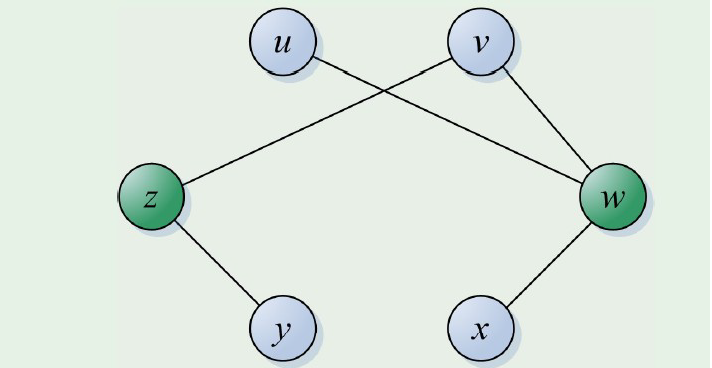
\includegraphics{image/Proof-of-Statute1.png}
        \caption{图中节点z, w组成的集合是一个顶点覆盖。}\label{fig:example}
    \end{figure}
\end{example}

\begin{definition}{最小顶点覆盖}
    最小顶点覆盖是图的一个顶点覆盖,并且其中的节点数最少。其形式化定义为:对于所有的顶点覆盖组成的集合 S = {$ S_1 $, $ S_2 $, ..., $ S_n $},最小顶点覆盖 $ S_m $,有 $ S_m \in $ S,∀ $ S_i \in $ S (i ≠ m), |$ S_i $| ≥ |$ S_m $|
\end{definition}


\section{独立集}

\begin{definition}{定义}
    图的一个顶点子集称为独立集,如果该子集中的任意两个项点在图中不相邻,也即没有边连接这两个点。
\end{definition}

\begin{definition}{形式化定义}
    给定图 G = (V,E),图节点集合 V,图边集合 E,图的一个独立集 S,S $\subseteq$ V,有 ∀u, v $\in$ S,(u,v) $\notin$ E
\end{definition}

\begin{example}
    如下图所示
	\begin{figure}[hbt]
        \centering
        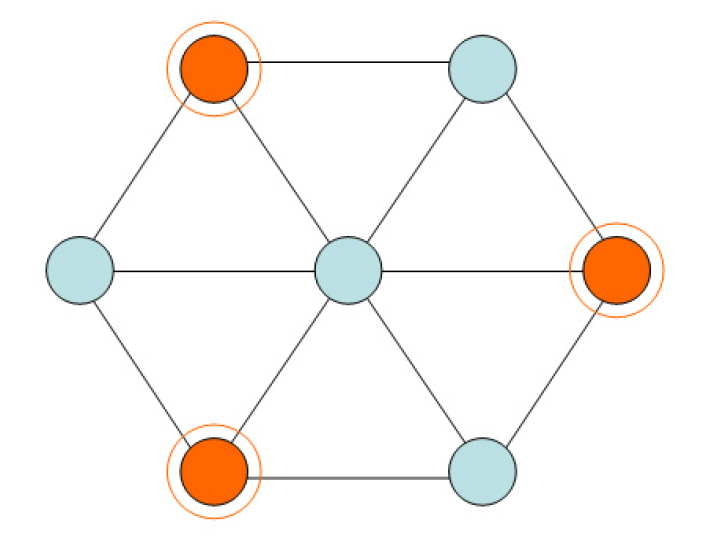
\includegraphics{image/Proof-of-Statute2.png}
        \caption{图中三个橙色的点构成图的一个独立集}\label{fig:example}
    \end{figure}
\end{example}

\begin{definition}{最大独立集}
    最大独立集是图的一个独立集,并且其中的节点数最多。其形式化定义为:对于图 G = (V,E) 所有的独立集组成的集合 S = {$ S_1 $, $ S_2 $, ..., $ S_n $},最大独立集 $ S_m $,有 $ S_m \in $ S,∀ $ S_i \in $ S (i ≠ m), |$ S_i $| $ \leq $ |$ S_m $|
\end{definition}


\section{顶点覆盖问题与独立集问题的相互规约}

\begin{theorem}{定理一}
    一个有n 个结点的图存在一个大小为k 的独立集,当且仅当这个图存在一个大小为n-k 的定点覆盖
\end{theorem}

\begin{proof}
    \begin{itemize}
        \item 当S是G的顶点覆盖时,V−S是G的独立集。当S是G的顶点覆盖时,V−S是G的独立集。也就是说对于(u,v) $\in$ E, u $\in$ S或者 v $\in$ S 或者 u, v $\in$ S,那么当只有 u $\in$ S时,可以将 v 放到独立集 S′ 中,对于 v 同理,如果 u, v $\in$ S,那么对于(u,v) 这条边的两个端点都不可以放入S′中。由于(u,v) 任意,根据上面的方法,u,v必然在S、S′中的一个集合中,因此 S $\cup$ S′= V,并且此时形成的独立集中任意两个点u′, v′, (u′, v′) ∉ E,否则在上面描述的方法中,u′, v′不可能全部放入独立集S′中。
        \item 当S是G的独立集时,V−S 是G的顶点覆盖。如果一个图G= (V , E) 有n个节点,它有一个k个节点的独立集S,则对于G中的任意一条边,其最多有一个端点在S中,也就是说对于(u,v) $\in$ E, u $\notin$ S或者 v $\notin$ S 或者 u, v $\notin$ S,那么当 u $\notin$ S时,可以将 u 放到顶点覆盖S′中,对于v同理,如果u,v∉S,那么可以将u,v都放入到顶点覆盖S′ 中。由于(u,v) 任意,根据上面的方法,u,v必然在S、S′中的一个集合中,因此 S $\cup$ S′= V,并且此时对于 ∀(u,v) $\in$ E,u $\in$ S′ 或者 v $\in$ S′ 或者 u, v $\in$ S′,否则根据上面描述的方法,必然没有遍历完所有的边。
    \end{itemize} 
\end{proof}


\begin{theorem}{定理二}
    一个有n 个结点的图存在一个最大独立集,当且仅当这个图存在一个最小定点覆盖
\end{theorem}

\begin{proof}
    对于一个图G= (V, E),其可能存在多个独立集,它们构成一个独立集集合S = {S1, S2, ..., Sn},我们可以找出其中结点数最多的一个独立集Sm,有k个节点,这就是这个图的最大独立集,那么由定理1,这个图就会有一个n-k 的一个顶点覆盖,这个顶点覆盖是图的最小顶点覆盖,可以使用反证法结合定理1 证明其正确性。
    同理,反过来我们可以找到图的一个大小为k 的最小顶点覆盖,那么根据定理1,可以得到一个大小为n-k 的独立集,这个独立集就是图的最大独立集,同样可以使用反证法结合定理1 证明其正确性。
\end{proof}